\documentclass[10pt]{article}

% Sort alphabetically by package name.
\usepackage[a4paper, margin=2cm]{geometry}
\usepackage{graphicx}
\usepackage{times}

\newcommand{\figref}[1]{Figure~\ref{fig:#1}}
\newcommand{\figlabel}[1]{\label{fig:#1}}

\title{Practical Graveyard Hashing}
\author{%Michael A. Bender \and   Removing Mike, at his request, until he determines whether he is contributing. 
        Bradley C. Kuszmaul \and
        William Kuszmaul}
\begin{document}
\maketitle

What are the requirements for a practical C++ hash table?
\begin{itemize}
\item Near-compatability with the C++ standard library hash table
  containers (\texttt{std::unordered\_set} and
  \texttt{std::unordered\_map}).  These are templated (parameterized)
  tables in which the user can specify a key, a hash function, and an
  equality function.  The tables support heterogeneous lookup (which
  allows you to construct something that can be hashed or compared to
  a key without actually constructing a key).  The stability
  properties can weaker.
    
\item Slightly weaker stability requirements than the C++ standard library containers.  This is about what happens to pointers to objects in the table.  In the standard library containers, you can get the pointer to an object that is stored in the table. Stability is the issue of how long that pointer remains valid.  For example, in the standard library
  \begin{itemize}
    \item If you destroy the table, any pointers into the table become invalid.
    \item There is also an \textit{iterator} that lets you step
      through all the values in a table.  An iterator value may
      reference a value in the table.  If you destroy the table, any
      existing iterators become invalid.
    \item If you erase an element from the table, then iterators and
      pointers that currently reference that element become invalid.
      Other iterators and pointers remain valid.
    \item If the table is rehashed (e.g., because it got too big),
      then all iterators become invalid, but all pointers remain valid.
   \end{itemize}

  In order to accommodate open-addressed hash tables, both Google and
  Facebook have adopted the modification to those rules:
  \begin{itemize}
  \item  If a table is rehashed, then its pointers also become invalid.
  \end{itemize}

   For example, the following code can result in undefined behavior
   (which means that your computer may crash or that all your files
   could be erased, among other things).
\begin{verbatim}
   // Define a set of integers
   flat_hash_map<int, int> table;
   
   table[42] += table[43];
\end{verbatim}
This can crash using the Google/Facebook tables, since
\texttt{table[42]} implicitly inserts a \texttt{42} into the table if
it isn't already there, and then `table[43]` implicitl inserts a
\texttt{43} into the table if isn't there.  (The order in which those
two inserts is performed is implementation-defined.  GCC does it in
one order, whereas Clang does it in the other).  The problem is that
the second insert may cause the table to rehash, invalidating the
pointer returned by the first insert, so when the \texttt{+=} operator
runs, it may be passed an invalid pointer.

  In order to prevent a table from being rehashed, people use the
  \texttt{reserve(n)} function, which guarantees that the hash table
  can hold $n$ values without rehashing (by rehashing the table
  immediately if necessary).  For example, if you write
\begin{verbatim}
  table.reserve(table.size() + 2);
  table[42] += table[43];
\end{verbatim}
  then you know that the table can absorb two more insertions without
  rehashing, and hence you know that the table won't be rehashed even
  if both 42 and 43 end up being inserted

  Note: Erasing from the table doesn't give you any credit.  If you
  reserve (table.size()+2) then erase one element, and then insert
  three, your table may get rehashed on the third insert.  The
  guarantee is ``No rehash will occur during the next \texttt{n -
    table.size()} insertions.''

\item Performance (cache locality).  One of the points of using these
  tables is to reduce the number of cache misses.  A chained hash
  table would have many cache misses for a lookup, whereas these
  tables use open addressing to try to reduce the number of cache
  misses.

\item Memory parsimony: Chained hash tables also have to pay memory
  for the pointers in the linked lists.  These tables try to save that
  memory by using open addressing.  The Google hash table can run at
  up to 7/8 full.  Unfortunately, in practice the Google hash tables
  run more like at 55\% to 65\% full, since when it rehashes it
  doubles the table size (it uses power-of-two table sizes) and
  reduces the load to 7/16 full.  This ought to produce a table that
  runs at 62\% full (if Benford's rule applies, you expect the
  geometric mean of the low- and hi- load factor.)  The calculations
  for the Facebook table are similar.

\item Not a requirement: Fine-grained parallelism.  Many authors data
  structures in the literature provide fine-grained lock-free
  parallelism, for example.  This is useless in a systems context,
  since there is no way to compose operations on that data structure
  with other operations to produce an atomic operation.  Real systems
  generally employ mutex locks, and require that the data structure be
  thread-compatible: that is, operations marked \texttt{const} may be
  called concurrently, and other operations need synchronization, such
  as a mutex, which is generally not part of the data structure.

\item Header-only: This isn't a requirement on the API, but an
  implementation that can be used as a set of headers is easier to
  integrate than an implementation that requirs building libraries and
  integrating them into a build system.  For example, the Facebook
  hash table uses CMake, and the Google table uses Bazel.  If you
  aren't already using the right build system, good luck.  A
  header-only library works by installing some header files to a
  directory and adding that directory to your compiler's search path.
\end{itemize}

Explain tombstones and graveyards.

Our table:
\begin{itemize}
\item Runs at 3/4 to 7/8 full (81\% on average if you believe in
  Benford's rule).  In our benchmarks, we use about 30\% less memory
  than the Facebook or Google tables.
\item Performance is about the same as the Facebook or Google tables.
\item High-water memory is 33\% lower.
\item Deamortized inserts to reduce the tail latencies.  (By 6 orders
  of magnitude).
\item Graveyard tombstones.
\end{itemize}

Results?
\begin{itemize}
  \item Graveyard tombstones show value at very high load factors (TODO).  At
    lower load factors, the difference is less significant.  
  \item How many tombstones do you need?  The theory says to do something like this:
    \begin{itemize}
    \item Rehash the table when it's 92.5\% full down to 90\% full.
    \item Make 5\% of the rehashed table be evenly-spaced graveyard
      tombstones, the other 5\% empty slots occur whereever there are
      holes after the insertion from the rehash.
    \end{itemize}
    We probably don't need so many graveyard tombstones, partly since
    rehashing is so fast compared to insertions.  We found that X\%
    was enough.
\end{itemize}

Experiments to run:
\begin{itemize}
\item Determine how much impact graveyard tombstones make.  May need to measure it at high load factors.

  It looks like graveyard hashing slows things down at 9092.  Inserts shouldn't be worse, so what's going on?  Maybe the wrong number of tombstones.

  Should we measure a wide variety of tombstone-counts at various high loads?
\end{itemize}

One bubble-sort step: prove that it is pretty good.

Hover workload: It looks like for a 3/4 full table, after doing t.size() hovers, the unsuccessful search cost has gone up from 1.018 probes to 1.276 probes.
For a 90\% full table, the unsuccessful search cost quickly rises from 1.2 to 1.6 after 10\%, then 2.2 after another 10\%.
Conclusion:  You should rehash after doing N hovers if you would have rehashed after doing N inserts.

\section{Experiments}

Hypothesis: Query-Optimized Graveyard hashing scales well to very high
load factors.

Todo: Define load factor.

Todo: Define ``an insertion-only workload'' is a workload in which the
only modifications to the table are insertions.  The workload may also
have queries.

Background: Most industrial-quality hash tables (e.g.,
\cite{Abseil,Folly} keep the load factor low.  For example, Google
(Abseil) and Facebook (F14) keep the load factor below $7/8$ (87.5\%),
and then double the table, reducing the load factor to $7/16$
(43.75\%).  If a workload is insertion-only, the expected load factor
would be thus some average of 87.5\% and 43.75\%.  If we believe
Benford's rule \cite{Benford} applies, then we take the geometric
average, and get 61.8\%.  We have heard that for real workloads at
google, the average load factor is closer to 55\%.  That's probably
because real workloads also remove items from tables, and removing an
item never causes a rehash.

One justification for using quadratic probing (Google) or double
hashing (Facebook) is that with traditional unordered linear probing
at high load factors, the probe lengths grow quadratically with $X$.
This rationale doesn't seem to actually justify the design decision
since the load factors are so low.

For this experiment we want to find out how well query-optimized
graveyard hashing scales as the load factor increases.  Here we
measured an insertion-only workload: We did the following:
\begin{itemize}
\item Create a table that is, say 90\%, full.
\item Rehash the table (at 90\% full) with tombstones (or without
  tombstones).  When using tombstones, we placed tombstones into half
  the remaining slots (5\% of the slots in this case).
\item Insert more items into the table.  The number of items is half
  the number of tombstones we placed.  (2.5\% in this case).  (In this
  case, the table is now 92.5\% full).
\item Measure the probe lengths.
\end{itemize}

\figref{probelengths} shows the result of our experiment.
The X axis is the final load factor (e.g., 92.5\% in the example above).  The $Y$ axis is the average probe length for a 
\figref{probelengths}(a) shows the average number of slots that must be
examined for a \textit{successful lookup}.  (Averaging over all the
values that are actually present in the table.)  What this shows is that lookup and insert scales very well for query-optimized graveyard hashing, and lookup scales well for traditional, but insert scales very badly for traditional (just the problem of finding an empty slot).

define: Traditional as stable ordered-linear probing.  Using the
search-distance hack so we can stop searching early.  (Without which,
without ordering, lookup would be quadratic.)  This isn't really
``Traditional'', so we probably need a better name.

\begin{figure}
\begin{center}
  \begin{tabular}{cc}
  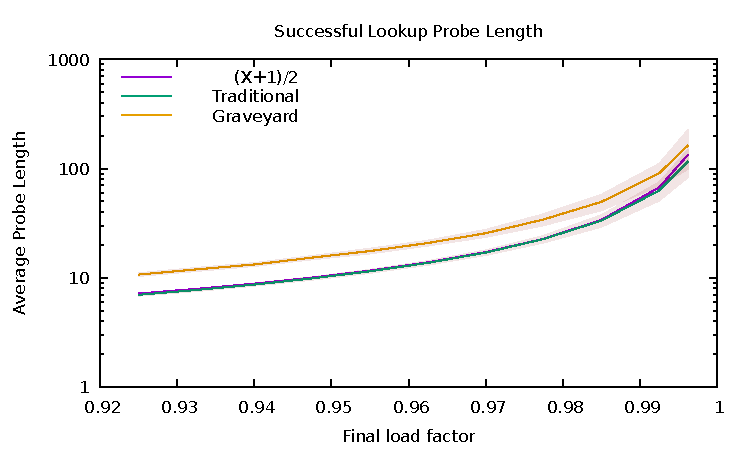
\includegraphics[width=75mm]{experiments/increasing-load-found}  &
  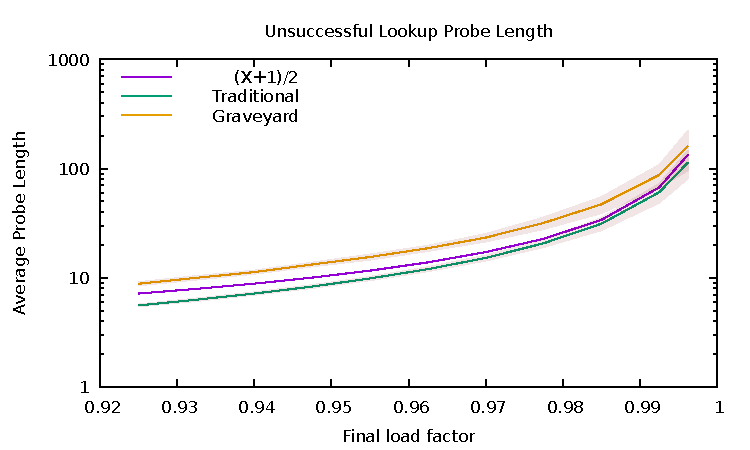
\includegraphics[width=75mm]{experiments/increasing-load-notfound}  \\
  \begin{minipage}{75mm}
    % TODO Get this font right.
    \footnotesize (a) Successful Lookup, comparing Graveyard,
    Traditional (both with 95\% confidence intervals shown, shaded),
    and Knuth's prediction $(X+1)/2$.
  \end{minipage}
  &
  \begin{minipage}{75mm}
    % TODO Get this font right.
    \footnotesize (a) Unsuccessful Lookup, comparing Graveyard,
    Traditional, and Knuth's prediction $(X+1)/2$.
  \end{minipage}
 
  \\
  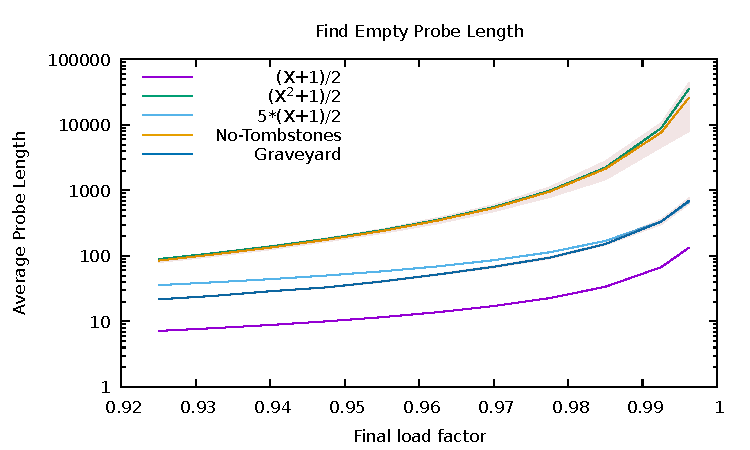
\includegraphics[width=75mm]{experiments/increasing-load-findempty} &
  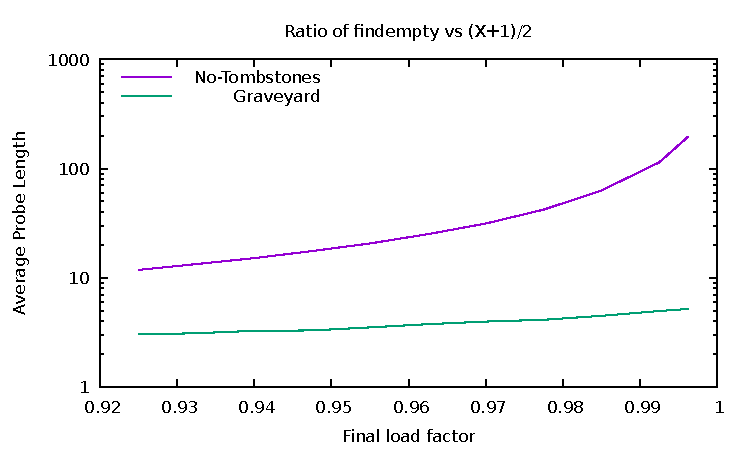
\includegraphics[width=75mm]{experiments/increasing-load-findempty-ratio}  \\
  \begin{minipage}{75mm}
    % TODO Get this font right.
    \footnotesize (a) Average probe length to find an empty slot for
    Graveyard, Traditional, and showing Knuth's $(X+1)/2$ prediction
    for lookup and $(X+1)/2$ prediction for insert.
  \end{minipage}
  &
  \begin{minipage}{75mm}
    % TODO Get this font right.
    \footnotesize (a) How much worse is find-empty than Knuth's
    lookup?  Graveyard is a small factor (staying near 4 even for very
    high load factors, traditional grows quickly.
  \end{minipage}
 
  \end{tabular}
\end{center}
\caption{How query-optimized graveyard hashing scales as the load factor increases.}
\figlabel{probelengths}
\end{figure}

\end{document}
